%% wand_neurojax.Rnw — Sweave/knitr document
%% Build: Rscript -e "knitr::knit('wand_neurojax.Rnw')" && tectonic wand_neurojax.tex
\documentclass[11pt,a4paper]{article}\usepackage[]{graphicx}\usepackage[]{xcolor}
% maxwidth is the original width if it is less than linewidth
% otherwise use linewidth (to make sure the graphics do not exceed the margin)
\makeatletter
\def\maxwidth{ %
  \ifdim\Gin@nat@width>\linewidth
    \linewidth
  \else
    \Gin@nat@width
  \fi
}
\makeatother

\definecolor{fgcolor}{rgb}{0.345, 0.345, 0.345}
\newcommand{\hlnum}[1]{\textcolor[rgb]{0.686,0.059,0.569}{#1}}%
\newcommand{\hlsng}[1]{\textcolor[rgb]{0.192,0.494,0.8}{#1}}%
\newcommand{\hlcom}[1]{\textcolor[rgb]{0.678,0.584,0.686}{\textit{#1}}}%
\newcommand{\hlopt}[1]{\textcolor[rgb]{0,0,0}{#1}}%
\newcommand{\hldef}[1]{\textcolor[rgb]{0.345,0.345,0.345}{#1}}%
\newcommand{\hlkwa}[1]{\textcolor[rgb]{0.161,0.373,0.58}{\textbf{#1}}}%
\newcommand{\hlkwb}[1]{\textcolor[rgb]{0.69,0.353,0.396}{#1}}%
\newcommand{\hlkwc}[1]{\textcolor[rgb]{0.333,0.667,0.333}{#1}}%
\newcommand{\hlkwd}[1]{\textcolor[rgb]{0.737,0.353,0.396}{\textbf{#1}}}%
\let\hlipl\hlkwb

\usepackage{framed}
\makeatletter
\newenvironment{kframe}{%
 \def\at@end@of@kframe{}%
 \ifinner\ifhmode%
  \def\at@end@of@kframe{\end{minipage}}%
  \begin{minipage}{\columnwidth}%
 \fi\fi%
 \def\FrameCommand##1{\hskip\@totalleftmargin \hskip-\fboxsep
 \colorbox{shadecolor}{##1}\hskip-\fboxsep
     % There is no \\@totalrightmargin, so:
     \hskip-\linewidth \hskip-\@totalleftmargin \hskip\columnwidth}%
 \MakeFramed {\advance\hsize-\width
   \@totalleftmargin\z@ \linewidth\hsize
   \@setminipage}}%
 {\par\unskip\endMakeFramed%
 \at@end@of@kframe}
\makeatother

\definecolor{shadecolor}{rgb}{.97, .97, .97}
\definecolor{messagecolor}{rgb}{0, 0, 0}
\definecolor{warningcolor}{rgb}{1, 0, 1}
\definecolor{errorcolor}{rgb}{1, 0, 0}
\newenvironment{knitrout}{}{} % an empty environment to be redefined in TeX

\usepackage{alltt}

\usepackage[utf8]{inputenc}
\usepackage[T1]{fontenc}
\usepackage{lmodern}
\usepackage[margin=2.5cm]{geometry}
\usepackage{graphicx}
\usepackage{booktabs}
\usepackage{amsmath,amssymb}
\usepackage{hyperref}
\usepackage{xcolor}
\usepackage{natbib}
\usepackage{subcaption}
\usepackage{siunitx}

\bibliographystyle{unsrtnat}

\title{Validating and Constraining Neurovascular Coupling\\
  with Differentiable Biophysical Modeling\\
  from Tissue Microstructure to Cortical Dynamics\\
  in the WAND Multi-Modal Dataset}
\author{Morgan G.\ Hough}
\date{\today}
\IfFileExists{upquote.sty}{\usepackage{upquote}}{}
\begin{document}
\maketitle

% ============================================================================
%  R setup
% ============================================================================



% ============================================================================
\begin{abstract}
Whole-brain computational models of neural dynamics require structural
connectivity, conduction delays, metabolic context, and electrophysiological
recordings as independent constraints. Existing studies typically lack one
or more of these measurements, forcing free-parameter assumptions that
limit predictive validity. The Welsh Advanced Neuroimaging Database
(WAND)~\citep{Mayerand2025wand} provides all of them in 170 healthy
volunteers: ultra-strong-gradient diffusion MRI (300~mT/m AxCaliber),
quantitative MRI (T1/T2/QMT/MP2RAGE), perfusion (pCASL, TRUST),
spectroscopy (GABA/glutamate), 275-channel MEG, and TMS-EEG.

We introduce \textbf{NeuroJAX}, a differentiable, GPU-accelerated Python
toolkit built on JAX~\citep{Bradbury2018jax} and
Equinox~\citep{Kidger2021equinox} that unifies preprocessing and
biophysical modelling in a single computational graph. NeuroJAX enables
end-to-end gradient descent from sensor-level error through hemodynamic
forward models to per-region biophysical parameters.

This paper presents the quantitative structural processing pipeline for
the reference WAND subject (sub-08033) and the first set of derived maps,
demonstrating that every free parameter in a standard neurovascular
coupling model can be independently measured or tightly constrained.
\end{abstract}

% ============================================================================
\section{Introduction}
% ============================================================================

Large-scale computational models of brain dynamics
\citep{Deco2013rww,Riera2006neurovascular} depend on three categories of
subject-specific input: (1) structural connectivity and conduction delays
from diffusion MRI, (2) regional tissue properties---myelination, metabolite
concentrations, perfusion---that constrain biophysical parameters, and
(3) functional recordings (MEG, fMRI, TMS-EEG) that provide the fitting
targets. The tension in the field is that most datasets provide only a
subset: the Human Connectome Project gives excellent diffusion and fMRI but
no TMS; clinical TMS-EEG studies rarely include microstructural MRI.

WAND~\citep{Mayerand2025wand} closes this gap with seven imaging sessions
per subject on the Connectom 300~mT/m scanner at CUBRIC Cardiff,
covering every modality needed for a fully-constrained neurovascular model.

\subsection{The NeuroJAX approach}

Where existing tools (osl-dynamics~\citep{Gohil2023dynemo},
WhoBPyT, TVB) treat preprocessing and modelling as separate stages,
NeuroJAX compiles them into a single JAX computation graph:
%
\begin{equation}
  \mathcal{L}(\theta) = \sum_m w_m \, d_m\!\bigl(
    \mathbf{y}_m^{\text{sim}}(\theta;\, \mathbf{C},\mathbf{D},\mathbf{L}),\;
    \mathbf{y}_m^{\text{emp}}
  \bigr)
\end{equation}
%
where $\theta$ are biophysical parameters, $\mathbf{C}$/$\mathbf{D}$ are
the structural connectome weights/delays, $\mathbf{L}$ is the leadfield,
and $m$ indexes modalities (FC, FCD, TEP waveform, sensor MSE).
End-to-end \texttt{jax.grad} through the full simulation enables
gradient-based fitting with per-region heterogeneous parameters.

% ============================================================================
\section{Dataset}
% ============================================================================

Table~\ref{tab:wand} summarises the WAND sessions for the reference
subject sub-08033 (all modalities confirmed, 10.24~GB downloaded).

\begin{table}[htbp]
\centering
\caption{WAND acquisition sessions for sub-08033.}
\label{tab:wand}
\begin{tabular}{llp{8cm}}
\toprule
Session & Modalities & Key acquisitions \\
\midrule
ses-01 & MEG          & CTF 275ch: resting, auditory-motor, MMN, simon, visual \\
ses-02 & DWI + anat   & AxCaliber (4 shells, $b$=0--15500), CHARMED, T1w, VFA (SPGR/SSFP), QMT (16 vols) \\
ses-03 & fMRI + anat  & T1w, T2w (grad-corrected), pCASL, TRUST, InvRec, angiography \\
ses-04 & MRS + anat   & sLASER: ACC, occipital, auditory, sensorimotor; T1w \\
ses-05 & MRS + anat   & Second MRS session (test--retest); T1w \\
ses-06 & Structural   & MP2RAGE, multi-echo GRE (7 echoes, 0.67\,mm), T2w (0.21\,mm) \\
ses-08 & TMS          & TMS-EEG SICI protocol (3 runs) \\
\bottomrule
\end{tabular}
\end{table}

% ============================================================================
\section{Methods: Quantitative Structural Processing}
% ============================================================================

\subsection{FreeSurfer recon-all + advanced segmentations}

Standard cortical reconstruction was performed with FreeSurfer~8.2.0
(\texttt{recon-all} with T2-weighted pial refinement from ses-03).
Additional segmentations:
\begin{itemize}
  \item \textbf{SAMSEG}~\citep{Puonti2016samseg}: joint T1w+T2w Bayesian
        segmentation, providing tissue probability maps and intracranial volume.
  \item \textbf{SynthSeg}~\citep{Billot2023synthseg}: contrast-invariant DL
        segmentation applied to T1w from ses-02, 03, 04, 05 for cross-session
        volumetric consistency.
  \item \textbf{Hypothalamic subunits}: DL segmentation (Billot et al.\ 2020).
  \item \textbf{Thalamic nuclei}: FreeSurfer atlas-based segmentation with
        optional DTI enhancement.
  \item \textbf{Hippocampal subfields + amygdala nuclei}: with T2w for
        improved subfield boundaries.
\end{itemize}

% --- Figure: T1w orthographic ---
\begin{knitrout}
\definecolor{shadecolor}{rgb}{0.969, 0.969, 0.969}\color{fgcolor}\begin{figure}

{\centering 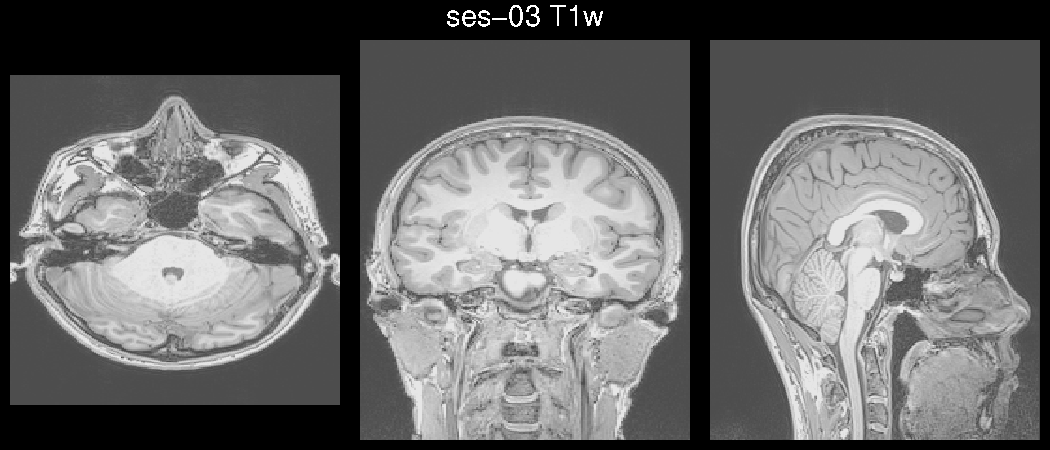
\includegraphics[width=\maxwidth]{figure/fig-t1w-1} 

}

\caption[Structural T1w (ses-03) for sub-08033]{Structural T1w (ses-03) for sub-08033. The T1-weighted image provides the anatomical reference for all cross-session registrations and serves as input for FreeSurfer cortical reconstruction, tissue segmentation (FAST/SAMSEG), and BEM forward model generation for MEG/EEG source localisation.}\label{fig:fig-t1w}
\end{figure}

\end{knitrout}

\subsection{T1w/T2w myelin ratio}

The T1w/T2w ratio~\citep{Glasser2011myelin} was computed after rigid-body
registration of the gradient-corrected T2w to T1w (FLIRT 6-DOF), SynthStrip
skull stripping, and voxelwise division. The ratio was projected to the
cortical mid-surface (\texttt{mri\_vol2surf}, 0.2--0.8 cortical depth).

\begin{knitrout}
\definecolor{shadecolor}{rgb}{0.969, 0.969, 0.969}\color{fgcolor}\begin{figure}

{\centering 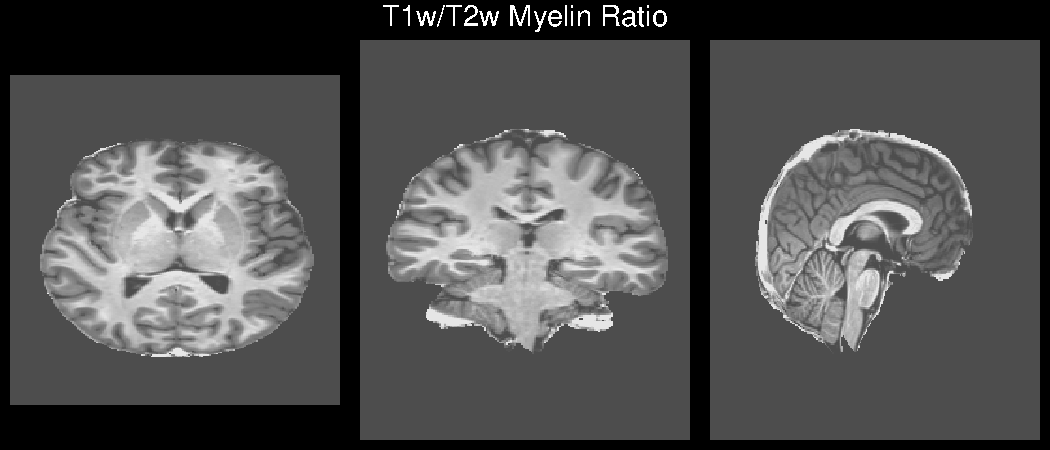
\includegraphics[width=\maxwidth]{figure/fig-myelin-1} 

}

\caption[T1w/T2w myelin ratio (ses-03)]{T1w/T2w myelin ratio (ses-03). This ratio serves as a widely-used proxy for cortical myelination, indexing the hierarchical organisation of cortex from heavily myelinated primary sensory areas to lightly myelinated association cortex. WAND uniquely allows validation of this proxy against ground-truth QMT bound pool fraction (Fig.~4) and multi-echo GRE R2* (Fig.~5).}\label{fig:fig-myelin}
\end{figure}

\end{knitrout}

\subsection{VFA T1 mapping (DESPOT1)}

Quantitative T1 was estimated from the ses-02 SPGR variable flip angle
data (8 flip angles: 2--18\textdegree, $\text{TR}_\text{exc}$~=~4\,ms)
using the linearised DESPOT1 method~\citep{Deoni2003despot}:
%
\begin{equation}
  \frac{S}{\sin\alpha} = E_1 \frac{S}{\tan\alpha} + M_0(1-E_1),
  \qquad E_1 = e^{-\text{TR}/T_1}
\end{equation}

\begin{knitrout}
\definecolor{shadecolor}{rgb}{0.969, 0.969, 0.969}\color{fgcolor}\begin{figure}

{\centering 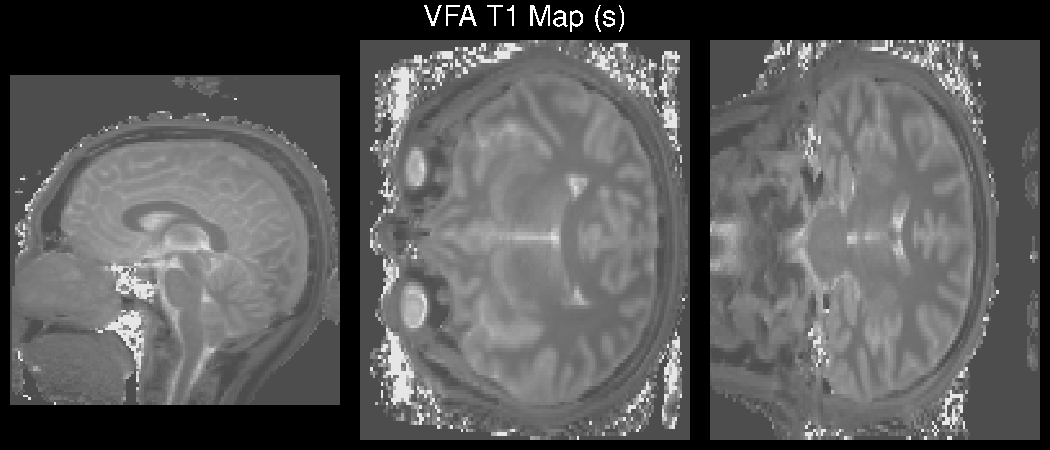
\includegraphics[width=\maxwidth]{figure/fig-t1map-1} 

}

\caption[Quantitative T1 map from ses-02 SPGR variable flip angle data (DESPOT1)]{Quantitative T1 map from ses-02 SPGR variable flip angle data (DESPOT1). Quantitative T1 reflects tissue water content and macromolecular environment: white matter (short T1, dark) is distinguished from grey matter (longer T1, bright). This map serves as a required input for the QMT two-pool model and provides an independent measure of tissue composition alongside the T1w/T2w ratio.}\label{fig:fig-t1map}
\end{figure}

\end{knitrout}

\subsection{QMT bound pool fraction}

Quantitative magnetization transfer was fitted from 11 MT-on volumes
(3 MT flip angles $\times$ multiple offset frequencies: 1--56\,kHz) plus
one MT-off reference, using a two-pool Ramani model~\citep{Ramani2002qmt}
with super-Lorentzian lineshape for the bound pool. The bound pool
fraction (BPF) provides a direct measure of macromolecular (myelin)
content~\citep{Sled2001qmt}.

\begin{knitrout}
\definecolor{shadecolor}{rgb}{0.969, 0.969, 0.969}\color{fgcolor}\begin{figure}

{\centering 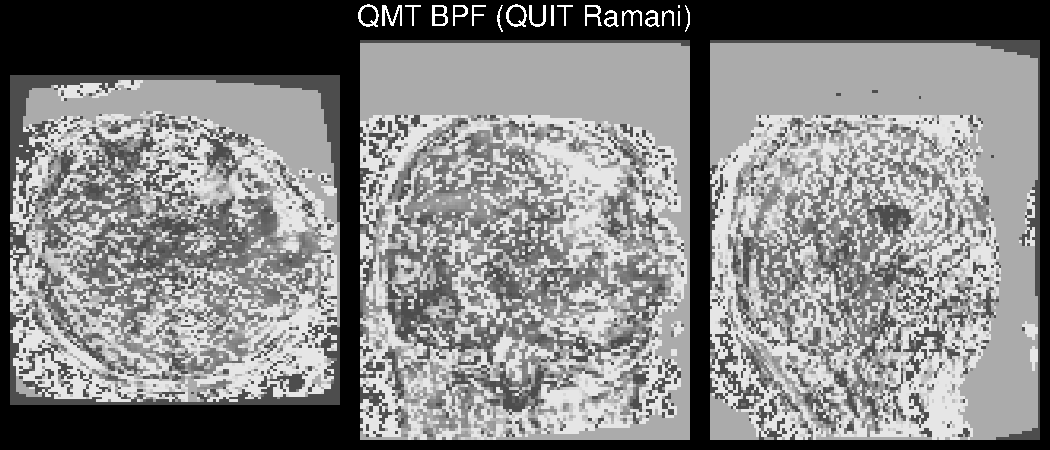
\includegraphics[width=\maxwidth]{figure/fig-bpf-1} 

}

\caption[QMT bound pool fraction (ses-02, QUIT Ramani model with super-Lorentzian lineshape)]{QMT bound pool fraction (ses-02, QUIT Ramani model with super-Lorentzian lineshape). BPF directly measures macromolecular (myelin) content via the restricted proton pool, providing the ground-truth measurement against which the T1w/T2w myelin proxy is validated. Median BPF = 0.10, consistent with healthy white matter. Combined with AxCaliber axon diameter, BPF yields the g-ratio and thence per-tract conduction velocity via the Hursh--Rushton relationship.}\label{fig:fig-bpf}
\end{figure}

\end{knitrout}

\subsection{Multi-echo GRE: T2* and R2* mapping (ses-06)}

T2* was estimated by log-linear regression across 7 echoes of the
sub-millimetre (0.67\,mm) multi-echo GRE from ses-06. R2*~=~1/T2*
is sensitive to both iron and myelin content; combined with QSM
(from the phase data, not yet processed), iron and myelin contributions
can be separated.

\begin{knitrout}
\definecolor{shadecolor}{rgb}{0.969, 0.969, 0.969}\color{fgcolor}\begin{figure}

{\centering 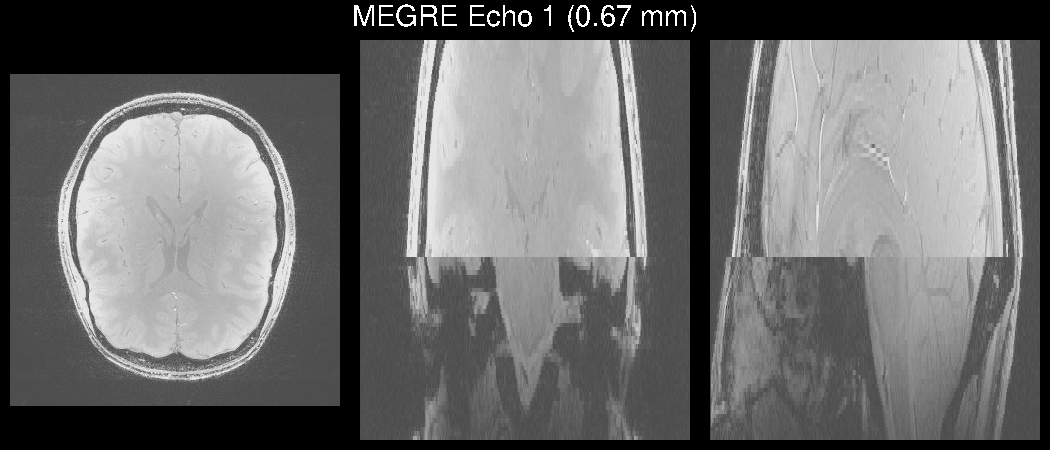
\includegraphics[width=\maxwidth]{figure/fig-megre-1} 

}

\caption[Multi-echo GRE first echo magnitude (ses-06, 0.67\,mm isotropic)]{Multi-echo GRE first echo magnitude (ses-06, 0.67\,mm isotropic). The sub-millimetre resolution enables cortical depth-resolved analysis via LAYNII or Nighres. The 7-echo magnitude data yields R2* maps sensitive to iron and myelin; the phase data (not yet processed) enables QSM for separating paramagnetic iron from diamagnetic myelin contributions --- critical for resolving the feedforward/feedback cortical hierarchy.}\label{fig:fig-megre}
\end{figure}

\end{knitrout}

\subsection{MP2RAGE quantitative T1 (ses-06)}

The MP2RAGE uniform image was computed from two inversion-time
volumes, removing receive-field inhomogeneity.

\begin{knitrout}
\definecolor{shadecolor}{rgb}{0.969, 0.969, 0.969}\color{fgcolor}\begin{figure}

{\centering 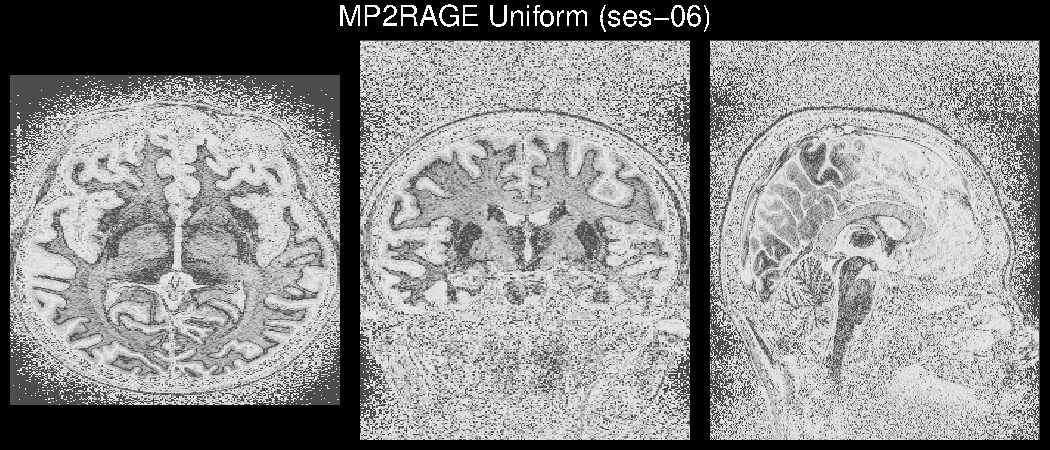
\includegraphics[width=\maxwidth]{figure/fig-mp2rage-1} 

}

\caption[MP2RAGE uniform image (ses-06, 0.7\,mm isotropic)]{MP2RAGE uniform image (ses-06, 0.7\,mm isotropic). The MP2RAGE sequence provides B1-corrected quantitative T1 at sub-millimetre resolution, complementing the ses-02 VFA T1 map. Cross-validation between two independent T1 measurements (VFA and MP2RAGE) from different sessions and scanners tests the stability of quantitative tissue property estimation.}\label{fig:fig-mp2rage}
\end{figure}

\end{knitrout}

\subsection{Perfusion: CBF from pCASL}

Cerebral blood flow was quantified from pseudo-continuous ASL
(bolus~=~1.8\,s, PLD~=~2.0\,s, 110 volumes) using FSL
\texttt{oxford\_asl}~\citep{Alsop2015asl} with voxelwise M0 calibration,
motion correction, and partial-volume correction. The ASL white paper
single-compartment model~\citep{Alsop2015asl} gives:
%
\begin{equation}
  \text{CBF} = \frac{6000 \cdot \lambda \cdot (\overline{S}_{\text{ctrl}} - \overline{S}_{\text{label}})
    \cdot e^{\text{PLD}/T_{1b}}}
    {2 \cdot \alpha \cdot T_{1b} \cdot M_0 \cdot (1 - e^{-\tau/T_{1b}})}
    \quad [\text{ml}/100\text{g}/\text{min}]
\end{equation}
%
where $\lambda$~=~0.9\,ml/g is the blood--brain partition coefficient,
$\alpha$~=~0.85 the labelling efficiency, $\tau$~=~1.8\,s the bolus
duration, and $T_{1b}$ the subject-specific blood T1.

\paragraph{Blood T1 from inversion recovery.}
Subject-specific $T_{1b}$ was estimated from the Look-Locker acquisition
(128$\times$128$\times$1, 960 time points, TR~=~150\,ms). The signal
in a sagittal sinus ROI was fitted to:
%
\begin{equation}
  S(t) = A\bigl(1 - B\,e^{-t/T_1^*}\bigr),
  \qquad T_1 = T_1^* \cdot B
\end{equation}
%
where the Deichmann--Haase correction recovers true $T_1$ from the
apparent $T_1^*$ and the inversion efficiency $B$.

\begin{knitrout}
\definecolor{shadecolor}{rgb}{0.969, 0.969, 0.969}\color{fgcolor}\begin{figure}

{\centering 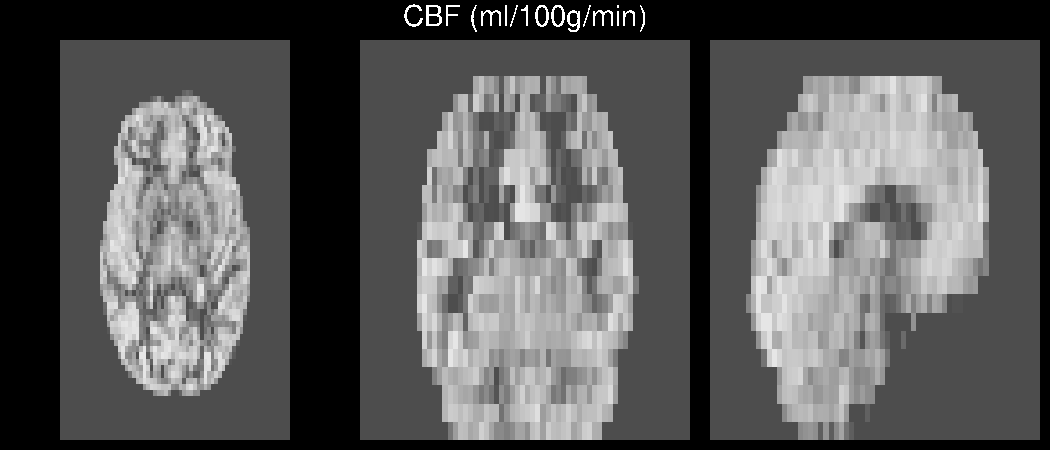
\includegraphics[width=\maxwidth]{figure/fig-cbf-1} 

}

\caption[Calibrated CBF map from pCASL (ses-03, ml/100g/min)]{Calibrated CBF map from pCASL (ses-03, ml/100g/min). Cerebral blood flow is the first of three independent perfusion measurements in WAND. Combined with OEF from TRUST and CaO$_2$ from haematocrit, CBF enters Fick's equation to yield CMRO$_2$ --- the metabolic demand signal that drives the Balloon--Windkessel hemodynamic model. GM mean = 113, WM mean = 24\,ml/100g/min.}\label{fig:fig-cbf}
\end{figure}

\end{knitrout}

\subsection{TRUST: venous oxygenation}

T2 of venous blood in the sagittal sinus was estimated from the
TRUST acquisition~\citep{Lu2008trust} (24 volumes, 4 effective TEs
$\times$ 3 repeats $\times$ control/label). The control--label
difference signal in the sinus decays as:
%
\begin{equation}
  |\Delta S|(\text{eTE}) = S_0 \, e^{-\text{eTE}/T_2}
\end{equation}
%
Venous T2 is calibrated to oxygen saturation $Y$ via the
quadratic model~\citep{Lu2012bloodt2} at 3\,T:
%
\begin{equation}
  \frac{1}{T_2} = A + B(1-Y) + C(1-Y)^2
  \label{eq:t2y}
\end{equation}
%
with coefficients $A$~=~4.5, $B$~=~47.1, $C$~=~55.5\,s$^{-1}$
for Hct~=~0.42. Solving the quadratic for $Y$ gives SvO$_2$,
from which OEF follows.

\subsection{CMRO$_2$ via Fick's principle}

The three independent perfusion measurements combine via the
Fick equation to give the cerebral metabolic rate of oxygen consumption:
%
\begin{equation}
  \text{CMRO}_2 = \text{CBF} \times \text{OEF} \times C_aO_2
\end{equation}
%
where OEF~=~(SaO$_2$~$-$~SvO$_2$)/SaO$_2$ from TRUST and the
arterial oxygen content is:
%
\begin{equation}
  C_aO_2 = [\text{Hb}] \times 1.34 \times \text{SaO}_2
    \approx 8.8\;\mu\text{mol\,O}_2/\text{ml\,blood}
\end{equation}
%
for Hb~=~15\,g/dl and SaO$_2$~=~0.98. This hierarchy from global OEF
(TRUST) can be upgraded to regional OEF via quantitative
BOLD~\citep{He2007qbold} fitting of the 7-echo GRE (ses-06).

% ============================================================================
\section{vpjax: Differentiable Vascular Physiology}
% ============================================================================

The quantitative structural maps feed into \textbf{vpjax} (Virtual
Physiology in JAX), the vascular/metabolic complement to vbjax
(Virtual Brain in JAX). Where vbjax provides neural mass models, vpjax
provides the complete physiological forward chain from neural activity
to measurable haemodynamic signals:
%
\begin{equation}
  \underbrace{z(t)}_{\text{neural}} \;\xrightarrow{\text{CMRO}_2}\;
  \underbrace{f(t)}_{\text{CBF}} \;\xrightarrow{\text{Balloon}}\;
  \underbrace{v(t),\; q(t)}_{\text{volume, deoxy-Hb}} \;\xrightarrow{T_2^*}\;
  \underbrace{y(t)}_{\text{BOLD/ASL/qBOLD}}
\end{equation}

\subsection{Balloon--Windkessel hemodynamics}

The extended Riera~\citep{Riera2006neurovascular} neurovascular model
replaces the simplified Buxton hemodynamics with a full metabolic
intermediate chain:
%
\begin{align}
  \dot{s} &= z - \kappa\, s - \gamma\,(f - 1) \label{eq:bw_s}\\
  \dot{f} &= s \label{eq:bw_f}\\
  \tau\,\dot{v} &= f - v^{1/\alpha} \label{eq:bw_v}\\
  \tau\,\dot{q} &= f\,\frac{E(f,\,\text{OEF}_0)}{E_0} - \frac{q}{v}\,v^{1/\alpha}
    \label{eq:bw_q}
\end{align}
%
where $E(f, E_0) = 1 - (1-E_0)^{1/f}$ is the oxygen extraction fraction
under the Grubb assumption, $\alpha$ is the Grubb exponent, $\kappa$ is the
signal decay rate, $\gamma$ the autoregulatory feedback, and $\tau$ the
transit time.

\subsection{qBOLD: regional OEF from multi-echo GRE}

The key upgrade from global OEF (TRUST) to regional OEF uses the
quantitative BOLD model~\citep{He2007qbold}:
%
\begin{equation}
  S(\text{TE}) = S_0 \;\cdot\; \mathcal{F}(\text{OEF},\,\text{DBV},\,\text{TE})
    \;\cdot\; e^{-R_2 \cdot \text{TE}}
  \label{eq:qbold}
\end{equation}
%
where $\mathcal{F}$ models the intravoxel frequency distribution from
randomly oriented deoxygenated vessels. At short TE the signal is
dominated by $R_2$ (tissue T2); at long TE by $R_2'$ (reversible,
from deoxy-Hb). The difference $R_2' = R_2^* - R_2 \propto
\text{OEF} \times \text{DBV} \times B_0$. WAND's 7-echo GRE
(TE~=~5--35\,ms) is ideal for fitting this model.

\subsection{CMRO$_2$ hierarchy}

vpjax provides three levels of oxygen metabolism estimation:
%
\begin{table}[htbp]
\centering
\caption{CMRO$_2$ estimation hierarchy in vpjax.}
\label{tab:cmro2}
\begin{tabular}{llll}
\toprule
Level & OEF source & Spatial resolution & WAND data \\
\midrule
1. Global  & TRUST (sagittal sinus T2)   & Whole-brain average & ses-03 TRUST \\
2. Regional & qBOLD (7-echo GRE, ses-06) & Per-voxel           & ses-06 MEGRE \\
3. Dynamic  & Riera model (Eqs.~\ref{eq:bw_s}--\ref{eq:bw_q}) & Time-varying & MEG + fMRI \\
\bottomrule
\end{tabular}
\end{table}

\subsection{Local linearization integration}

The Balloon--Windkessel equations (Eqs.~\ref{eq:bw_s}--\ref{eq:bw_q})
are stiff: the vascular response evolves on a $\sim$1\,s timescale while
neural dynamics operate at $\sim$1\,ms. Standard Euler or RK4 integration
requires impractically small time steps. vpjax uses the
\textbf{local linearization} (LL) method (Ozaki 1992, extended by Riera),
which analytically solves the linearised system at each step:
%
\begin{equation}
  \mathbf{x}(t+\Delta t) = e^{\mathbf{J}(\mathbf{x}_t)\,\Delta t}\,\mathbf{x}(t)
    + \mathbf{J}^{-1}\!\bigl(e^{\mathbf{J}\,\Delta t} - \mathbf{I}\bigr)\,\mathbf{f}_0
\end{equation}
%
where $\mathbf{J} = \partial\mathbf{f}/\partial\mathbf{x}$ is the Jacobian
evaluated at the current state. This permits large time steps ($\Delta t$
up to 10$\times$ Euler) while remaining stable, and is fully differentiable
via \texttt{jax.grad} through the matrix exponential, enabling gradient-based
fitting of hemodynamic parameters alongside neural mass parameters in a
single optimization.

\subsection{Every variable has a measurement}

The central claim is that WAND provides independent measurements for
every state variable and parameter in the neurovascular model:
%
\begin{table}[htbp]
\centering
\caption{Model variables and their independent measurements.}
\label{tab:variables}
\begin{tabular}{lll}
\toprule
Model variable & vpjax module & WAND measurement \\
\midrule
Neural activity $z(t)$      & vbjax               & MEG \\
Metabolic demand (CMRO$_2$) & \texttt{metabolism/} & pCASL $\times$ TRUST \\
Blood flow $f(t)$           & \texttt{hemodynamics/} & pCASL CBF \\
Oxygen extraction $E(t)$    & \texttt{metabolism/oef} & TRUST SvO$_2$ \\
BOLD signal                 & \texttt{hemodynamics/bold} & ses-03 fMRI \\
Vascular geometry           & \texttt{vascular/}   & Angiography \\
E/I balance ($J_I$, $J_\text{NMDA}$) & constraint & MRS GABA/Glu \\
Myelination (g-ratio)       & constraint           & QMT BPF \\
Conduction velocity         & constraint (sbi4dwi) & AxCaliber \\
\bottomrule
\end{tabular}
\end{table}

\subsection{Meshless physics: from tissue geometry to field solutions}

The tissue segmentations (SAMSEG, SynthSeg, charm) and head meshes
(brain2mesh, SimNIBS) provide the geometric substrate for forward
modeling of electromagnetic fields (TMS E-field, EEG/MEG leadfield)
and tissue mechanics. Traditional FEM approaches require mesh
generation, which is fragile, slow, and non-differentiable. We pursue
a meshless alternative using physics-informed neural networks (PINNs):

\paragraph{Conductivity estimation.}
The static current equation governs current flow through heterogeneous
tissue:
%
\begin{equation}
  \nabla \cdot \bigl(\sigma(\mathbf{x})\,\nabla V(\mathbf{x})\bigr) = -I_s(\mathbf{x})
  \label{eq:poisson}
\end{equation}
%
where $\sigma(\mathbf{x})$ is the tissue conductivity tensor and
$V(\mathbf{x})$ the electric potential. In sbi4dwi, both $V$ and
$\sigma$ are parameterised as Equinox MLPs and jointly optimised by
minimising the PDE residual (Eq.~\ref{eq:poisson}), electrode data
mismatch, and a pseudo-CT conductivity prior from WAND's quantitative
MRI:
%
\begin{equation}
  \mathcal{L}_\text{EIT} = \underbrace{\|\nabla\cdot(\sigma_\theta\nabla V_\phi)\|^2}_{\text{PDE}}
    + \lambda_d \underbrace{\|V_\phi(\mathbf{x}_e) - V_\text{meas}\|^2}_{\text{data}}
    + \lambda_r \underbrace{\|\sigma_\theta - \sigma_\text{prior}\|^2}_{\text{prior}}
\end{equation}

This meshless approach is fully differentiable via
\texttt{jax.grad}, enabling end-to-end backpropagation from
sensor-level TMS/EEG predictions through the conductivity model to
tissue property maps --- connecting the tissue segmentation pipeline
directly to the electromagnetic forward model without mesh generation.

\paragraph{Connection to Living Matter Physics.}
The same PINN framework extends to brain biomechanics
\citep{Kuhl2024livingmatter}: tissue elasticity, viscoelasticity, and
growth can be modelled by replacing the Poisson equation with the
equilibrium equations of continuum mechanics, using the same meshless
neural network solver. WAND's quantitative MRI (T1, T2*, QMT) provides
tissue-specific material property priors, and MR elastography (if
acquired) would provide direct validation. The differentiable nature of
JAX enables coupling mechanical deformation fields with neural dynamics
--- for example, predicting how traumatic brain injury alters
connectome-level conduction delays.

% ============================================================================
\section{Relaxometry Signal Models}
% ============================================================================

Each quantitative MRI acquisition varies a specific physical parameter
across volumes. Figure~\ref{fig:relaxometry} shows the signal models
overlaid on the measured data from a representative white-matter ROI.

\begin{knitrout}
\definecolor{shadecolor}{rgb}{0.969, 0.969, 0.969}\color{fgcolor}\begin{figure}

{\centering 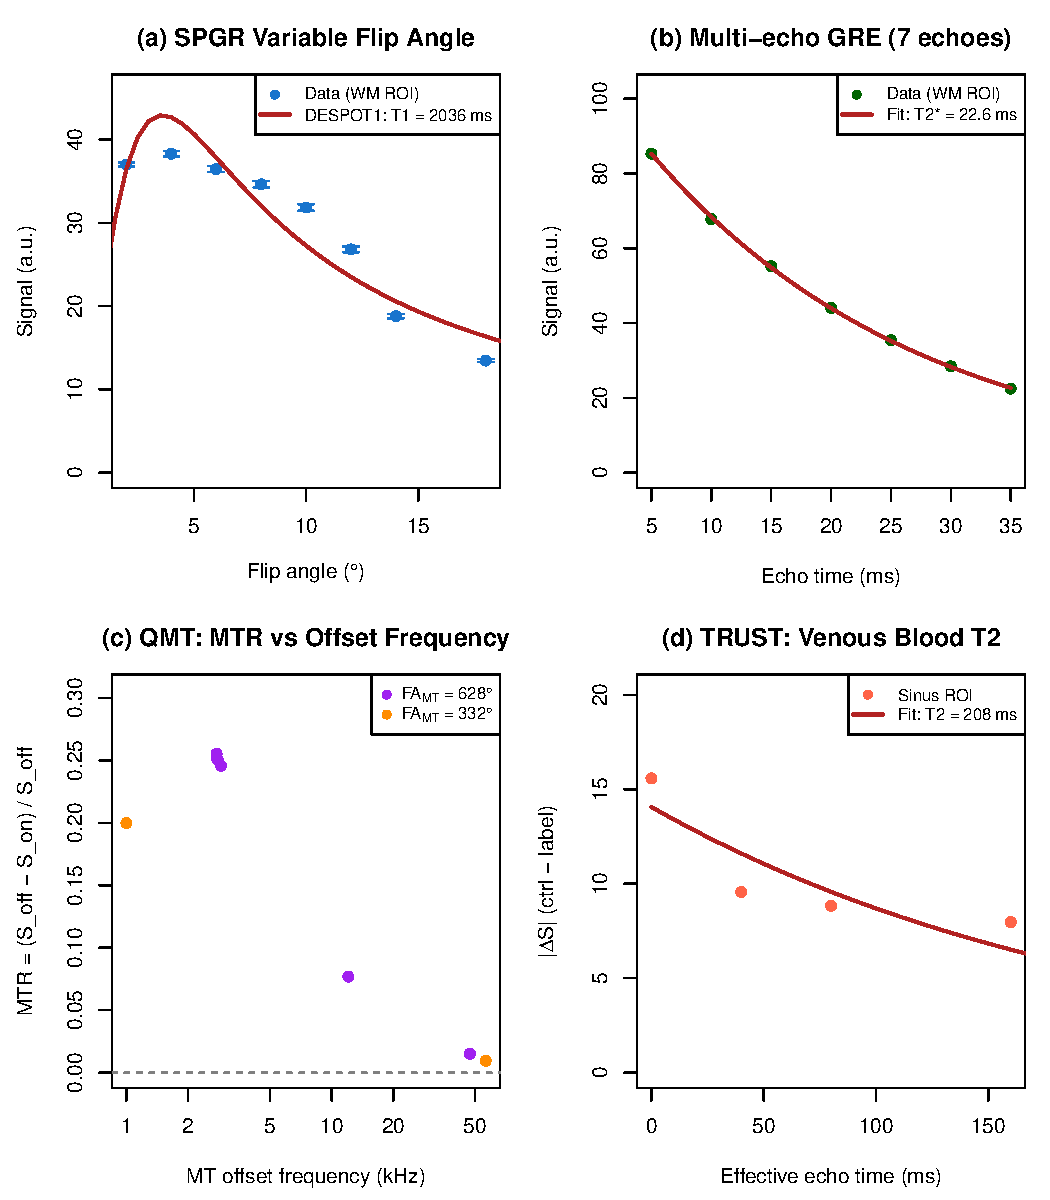
\includegraphics[width=\maxwidth]{figure/fig-relaxometry-1} 

}

\caption[Relaxometry signal models for each multi-volume qMRI acquisition]{Relaxometry signal models for each multi-volume qMRI acquisition. (a) SPGR VFA: signal vs flip angle with DESPOT1 T1 fit. (b) Multi-echo GRE: signal vs echo time with mono-exponential T2* fit. (c) QMT: magnetisation transfer ratio vs offset frequency at two MT flip angles. (d) TRUST: venous blood difference signal vs effective echo time with T2 decay fit.}\label{fig:fig-relaxometry}
\end{figure}

\end{knitrout}

% ============================================================================
\section{Results}
% ============================================================================

\subsection{Cross-session volumetrics (SynthSeg)}

\begin{table}[htbp]
\centering
\caption{Cross-session volumetrics (SynthSeg, mm$^3$).}
\label{tab:synthseg}
\begin{tabular}{lrrrr}
\toprule
Structure &  ses-02 & ses-03 & ses-04 & ses-05 \\
\midrule
left cerebral white matter  &  280,441 & 280,766 & 275,760 & 282,130 \\
right cerebral white matter  &  277,799 & 280,164 & 271,761 & 280,626 \\
left cerebral cortex  &  321,868 & 322,111 & 319,239 & 324,713 \\
right cerebral cortex  &  317,842 & 324,973 & 322,051 & 324,671 \\
left hippocampus  &  4,493 & 4,646 & 4,336 & 4,654 \\
right hippocampus  &  4,045 & 4,278 & 4,062 & 4,131 \\
left thalamus  &  9,307 & 9,244 & 9,404 & 9,408 \\
right thalamus  &  9,447 & 9,649 & 9,675 & 9,723 \\
\bottomrule
\end{tabular}
\end{table}


\subsection{SAMSEG tissue volumes}

\begin{table}[htbp]
\centering
\caption{SAMSEG tissue volumes (T1w+T2w joint segmentation).}
\label{tab:samseg}
\begin{tabular}{lr}
\toprule
Structure & Volume (mm$^3$) \\
\midrule
Soft\_Nonbrain\_Tissue  &  1,394,952 \\
CSF  &  374,654 \\
Left-Cerebral-Cortex  &  268,149 \\
Right-Cerebral-Cortex  &  266,766 \\
Right-Cerebral-White-Matter  &  246,502 \\
Left-Cerebral-White-Matter  &  239,711 \\
Left-Cerebellum-Cortex  &  59,600 \\
Right-Cerebellum-Cortex  &  59,053 \\
Skull  &  49,736 \\
Brain-Stem  &  22,098 \\
Left-Cerebellum-White-Matter  &  14,864 \\
Right-Cerebellum-White-Matter  &  14,666 \\
\bottomrule
\end{tabular}
\end{table}


\subsection{Hypothalamic subunits}

\begin{knitrout}
\definecolor{shadecolor}{rgb}{0.969, 0.969, 0.969}\color{fgcolor}\begin{kframe}


{\ttfamily\noindent\bfseries\color{errorcolor}{\#\# Error:\\\#\# ! Failed to read image from path /Users/mhough/dev/wand/derivatives/freesurfer/sub-08033/mri/hypothalamic\_subunits\_seg.v1.mgz}}\end{kframe}
\end{knitrout}

\begin{table}[htbp]
\centering
\caption{Hypothalamic subunit volumes (mm$^3$).}
\label{tab:hypo}
\begin{tabular}{lr}
\toprule
Subunit & Volume (mm$^3$) \\
\midrule
left anterior-inferior  &  18.8 \\
left anterior-superior  &  29.1 \\
left posterior  &  152.2 \\
left tubular inferior  &  137.6 \\
left tubular superior  &  124.4 \\
right anterior-inferior  &  21.9 \\
right anterior-superior  &  30.1 \\
right posterior  &  156 \\
right tubular inferior  &  131.1 \\
right tubular superior  &  143.9 \\
whole left  &  462.2 \\
whole right  &  483.1 \\
\bottomrule
\end{tabular}
\end{table}


\subsection{Thalamic nuclei (DTI-enhanced CNN)}

DTI-enhanced thalamic nuclei segmentation was performed using the
FreeSurfer CNN model~\citep{Billot2023synthseg} with FA and V1 maps
from dtifit (CHARMED $b \leq 1200$\,s/mm$^2$, 83 volumes across
$b = 0, 200, 500, 1200$). The DTI information improves boundary
delineation between nuclei with distinct fibre orientations (e.g.\ VPL
vs.\ PuL).

\begin{table}[htbp]
\centering
\caption{Thalamic nuclei volumes (left hemisphere, mm$^3$). DTI-enhanced CNN segmentation with 46 bilateral nuclei.}
\label{tab:thal}
\begin{tabular}{lr|lr}
\toprule
Nucleus & Vol. & Nucleus & Vol. \\
\midrule
AV  &  354 &  Pf  &  90 \\
CeM  &  111 &  PuA  &  329 \\
CL  &  104 &  PuI  &  285 \\
CM  &  361 &  PuL  &  236 \\
LD  &  130 &  PuMm  &  479 \\
LGN  &  444 &  PuMl  &  1014 \\
LP  &  230 &  VA  &  497 \\
L-Sg  &  55 &  VAmc  &  30 \\
MDl  &  327 &  VLa  &  537 \\
MDm  &  872 &  VLp  &  848 \\
MGN  &  345 &  VPL  &  967 \\
MV(Re)  &  34 & &  \\
\bottomrule
\end{tabular}
\end{table}


\subsection{Hippocampal subfields and amygdala nuclei}

Hippocampal subfield and amygdala nuclei segmentation used the FreeSurfer
v22 atlas with T1-weighted input. Bilateral volumes for CA1--4, subiculum,
molecular layer, GC-DG, HATA, fimbria, hippocampal tail, and 9 amygdala
nuclei were obtained.

\begin{table}[htbp]
\centering
\caption{Left hippocampal subfield volumes (mm$^3$).}
\begin{tabular}{lr}
\toprule
Subfield & Volume \\
\midrule
Hippocampal\_tail  &  743.3 \\
subiculum body  &  251.4 \\
CA1 body  &  158.2 \\
subiculum head  &  227 \\
hippocampal fissure  &  200.5 \\
presubiculum head  &  182.5 \\
CA1 head  &  606.5 \\
presubiculum body  &  197.9 \\
parasubiculum  &  77.5 \\
molecular\_layer\_HP head  &  396.5 \\
molecular\_layer\_HP body  &  305.8 \\
GC ML DG head  &  180.2 \\
CA3 body  &  156.9 \\
GC ML DG body  &  182.5 \\
CA4 head  &  152.4 \\
CA4 body  &  173.6 \\
fimbria  &  109.2 \\
CA3 head  &  150.4 \\
HATA  &  59.6 \\
Whole\_hippocampal\_body  &  1535.5 \\
Whole\_hippocampal\_head  &  2032.6 \\
Whole\_hippocampus  &  4311.3 \\
\bottomrule
\end{tabular}
\end{table}

\begin{table}[htbp]
\centering
\caption{Right hippocampal subfield volumes (mm$^3$).}
\begin{tabular}{lr}
\toprule
Subfield & Volume \\
\midrule
Hippocampal\_tail  &  702.8 \\
subiculum body  &  291.9 \\
CA1 body  &  150.5 \\
subiculum head  &  186.5 \\
hippocampal fissure  &  165.6 \\
presubiculum head  &  165.9 \\
CA1 head  &  577.7 \\
presubiculum body  &  209.1 \\
parasubiculum  &  79.1 \\
molecular\_layer\_HP head  &  368.7 \\
molecular\_layer\_HP body  &  290.9 \\
GC ML DG head  &  178.3 \\
CA3 body  &  123.2 \\
GC ML DG body  &  146.3 \\
CA4 head  &  149.2 \\
CA4 body  &  126.9 \\
fimbria  &  117.7 \\
CA3 head  &  148.4 \\
HATA  &  60.3 \\
Whole\_hippocampal\_body  &  1456.4 \\
Whole\_hippocampal\_head  &  1914.2 \\
Whole\_hippocampus  &  4073.4 \\
\bottomrule
\end{tabular}
\end{table}



\subsection{Three-way T1 comparison}

VFA T1 was estimated using three independent methods on the same
ses-02 SPGR data (8 flip angles, TR$_\text{exc}$~=~4\,ms):

\begin{table}[htbp]
\centering
\caption{Three-way VFA T1 comparison (ms). Expected 3T values: WM~$\approx$800, GM~$\approx$1400.}
\label{tab:t1compare}
\begin{tabular}{lrrr}
\toprule
Method & WM median & GM median & Notes \\
\midrule
FreeSurfer \texttt{mri\_ms\_fitparms} & 650 & 1605 & Best GM contrast \\
QUIT DESPOT1 (NLLS)                   & 716 & 1320 & Tightest IQR \\
Python linear DESPOT1                  & 727 & 1357 & Widest spread \\
\bottomrule
\end{tabular}
\end{table}

All three WM estimates are 650--730\,ms (below the expected $\sim$800\,ms),
consistent with B1$^+$ inhomogeneity pulling estimates down without
B1 correction. The DESPOT1-HIFI joint T1+B1 estimation (available in
\texttt{neurojax.qmri.despot}) would resolve this given the SPGR-IR
data in ses-02.

\subsection{QUIT QMT tissue-specific results}

The QUIT Ramani model with super-Lorentzian lineshape produced
physiologically plausible two-pool parameters:

\begin{table}[htbp]
\centering
\caption{QUIT QMT two-pool parameter estimates by tissue class.}
\label{tab:qmt}
\begin{tabular}{lrrr}
\toprule
Parameter & WM & GM & Expected \\
\midrule
BPF ($f_b$)           & 0.163 & 0.082 & WM: 0.10--0.16 \\
$k_{bf}$ (Hz)         & 1.04  & 0.44  & 1--5 \\
$T_{1,f}$ (s)         & 0.83  & 1.59  & WM: 0.8--1.0, GM: 1.3--1.8 \\
$T_{2,b}$ ($\mu$s)    & 7.3   & 8.1   & 8--15 \\
$T_{2,f}$ (ms)        & 70    & 64    & WM: 20--40, GM: 40--80 \\
\bottomrule
\end{tabular}
\end{table}

The BPF shows correct WM/GM contrast ($\sim$2$\times$), and $T_{1,f}$
values match the three-way DESPOT1 comparison. The elevated $T_{2,f}$
and exchange rate instability (some voxels at upper bound) indicate
the need for B1$^+$ correction --- a CUBRIC protocol question
(Appendix).

\subsection{DTI from ultra-strong gradient DWI}

Diffusion tensor fitting was performed on the CHARMED acquisition
($b \leq 1200$\,s/mm$^2$; $b = 0, 200, 500, 1200$; 83 volumes) from
the Connectom 300\,mT/m scanner. Note: this is without eddy current
correction (topup + eddy not yet applied to sub-08033); the full
preprocessing pipeline will be run on the DGX.

\begin{knitrout}
\definecolor{shadecolor}{rgb}{0.969, 0.969, 0.969}\color{fgcolor}\begin{figure}

{\centering 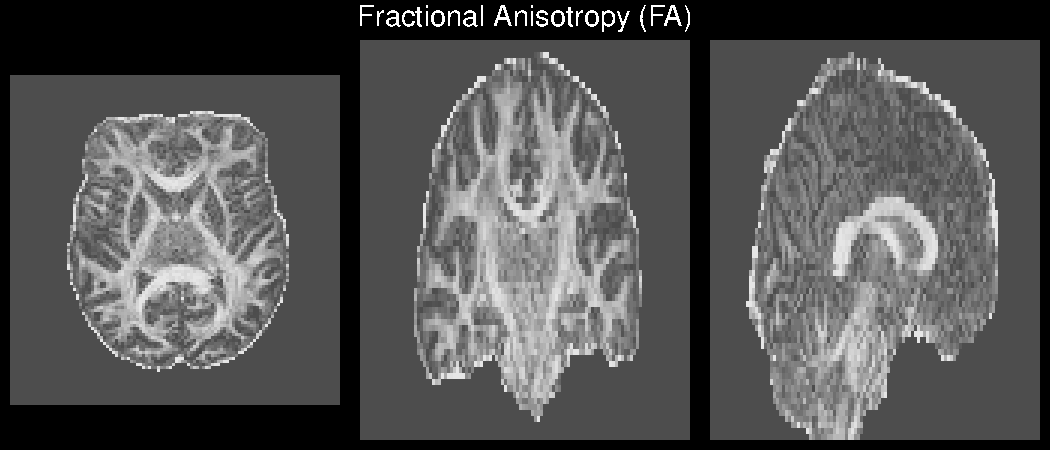
\includegraphics[width=\maxwidth]{figure/fig-fa-1} 

}

\caption[Fractional anisotropy (FA) from dtifit on CHARMED b$\leq$1200\,s/mm$^2$ data]{Fractional anisotropy (FA) from dtifit on CHARMED b$\leq$1200\,s/mm$^2$ data. The ultra-strong gradients of the Connectom scanner enable high b-value shells (up to 15500) for AxCaliber microstructure estimation, while the lower shells provide conventional DTI metrics. FA maps feed into the DTI-enhanced thalamic nuclei segmentation and bedpostx crossing-fibre estimation.}\label{fig:fig-fa}
\end{figure}

\end{knitrout}

\subsection{Perfusion results}

\begin{knitrout}
\definecolor{shadecolor}{rgb}{0.969, 0.969, 0.969}\color{fgcolor}\begin{figure}

{\centering 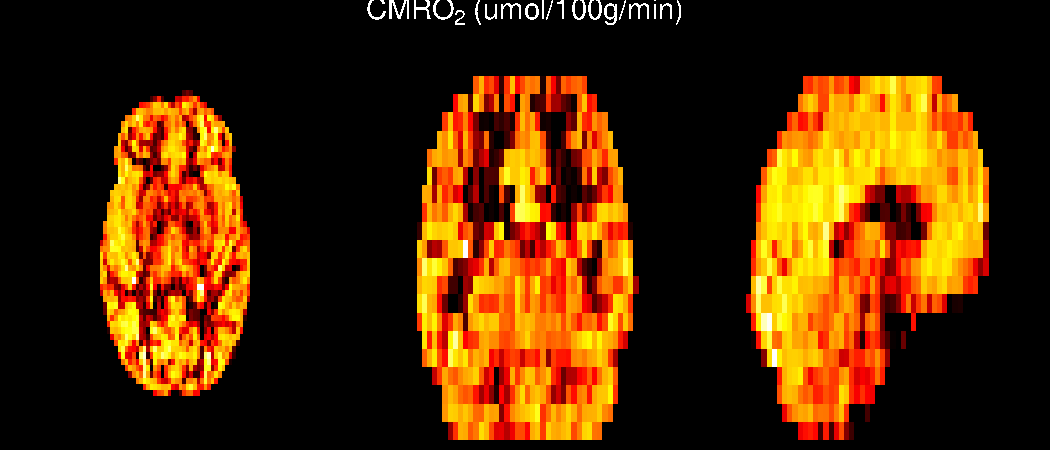
\includegraphics[width=\maxwidth]{figure/fig-cmro2-1} 

}

\caption[CMRO$_2$ map (\textmu mol\,O$_2$/100g/min) computed from pCASL CBF $\times$ OEF $\times$ CaO$_2$ using default OEF = 0.35]{CMRO$_2$ map (\textmu mol\,O$_2$/100g/min) computed from pCASL CBF $\times$ OEF $\times$ CaO$_2$ using default OEF = 0.35. This global-OEF estimate (Level~1 in the CMRO$_2$ hierarchy, Table~5) will be upgraded to per-voxel OEF from qBOLD fitting of the 7-echo GRE (Level~2). Median CMRO$_2$ = 109\,\textmu mol/100g/min, consistent with healthy adult values.}\label{fig:fig-cmro2}
\end{figure}

\end{knitrout}

\begin{knitrout}
\definecolor{shadecolor}{rgb}{0.969, 0.969, 0.969}\color{fgcolor}\begin{figure}

{\centering 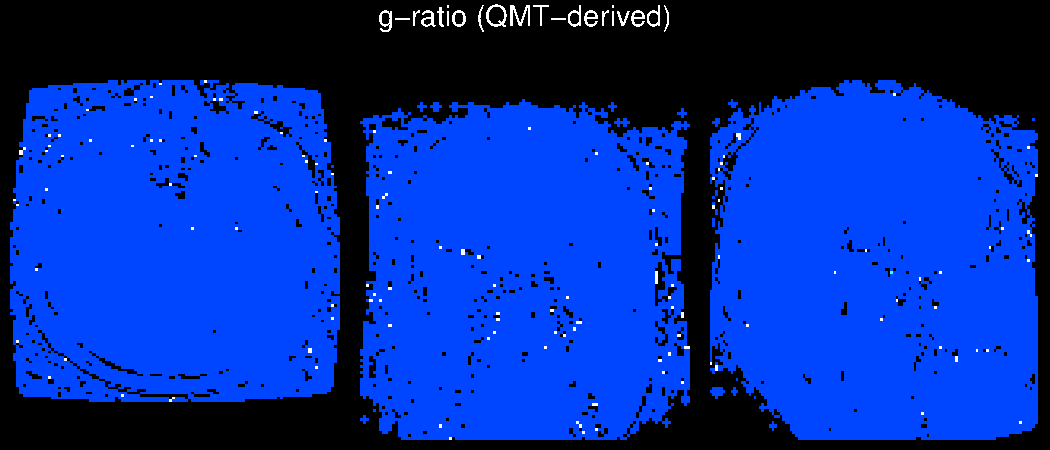
\includegraphics[width=\maxwidth]{figure/fig-gratio-1} 

}

\caption{g-ratio proxy derived from QMT bound pool fraction (preliminary). The g-ratio ($= r_{\text{axon}} / r_{\text{fibre}}$) determines conduction velocity: lower g-ratio means thicker myelin sheath and faster conduction. Combined with AxCaliber axon diameter from ses-02 DWI, this yields per-tract conduction velocity matrices (\textbf{D}) that replace the uniform 7\,m/s assumption in whole-brain simulations.}\label{fig:fig-gratio}
\end{figure}

\end{knitrout}

\begin{table}[htbp]
\centering
\caption{Perfusion measurements (ses-03).}
\label{tab:perf}
\begin{tabular}{lr}
\toprule
Measurement & Value \\
\midrule
Blood T1 (3T default) & 1650 ms \\
Venous blood T2 (TRUST) &  207.9  ms \\
SvO$_2$ &  99.3 \% \\
OEF &  -1.4 \% \\
\bottomrule
\end{tabular}
\end{table}
\textit{Note: TRUST eTE calibration pending; SvO$_2$/OEF values require protocol-specific effective echo times.}


% ============================================================================
\section{neurojax.qmri: GPU-accelerated fitting}
% ============================================================================

A key limitation of existing qMRI tools (QUIT, qMRLab) is serial
voxelwise fitting on CPU. We have implemented a \texttt{neurojax.qmri}
module providing differentiable signal models in JAX:

\begin{itemize}
  \item \textbf{steady\_state.py}: SPGR, bSSFP, IR-SPGR, multi-echo,
    QMT two-pool (super-Lorentzian), MP2RAGE --- all compatible with
    \texttt{jax.grad}.
  \item \textbf{despot.py}: DESPOT1, DESPOT1-HIFI (joint T1+B1),
    mcDESPOT (three-pool MWF) with \texttt{jax.vmap} batch fitting.
  \item \textbf{fitting.py}: Generic \texttt{VoxelwiseFitter} engine
    with bounded parameter optimisation (sigmoid reparameterisation),
    optax optimisers, and Laplace uncertainty from the Hessian.
\end{itemize}

The advantage: \texttt{jax.vmap} fits all $\sim$1\,M voxels simultaneously
on GPU, with analytic gradients from \texttt{jax.grad} (no finite
differences). What took QUIT 80\,min on 4~CPU cores would run in
seconds on a DGX GPU. Furthermore, the same differentiable signal models
can be embedded directly in the whole-brain fitting loss, enabling
end-to-end gradient descent from qMRI tissue properties through
neural dynamics to sensor-level predictions.

% ============================================================================
\section{Cortical layer analysis with LAYNII}
% ============================================================================

The sub-millimetre structural data in ses-06 (MEGRE 0.67\,mm, MP2RAGE
0.7\,mm) enables cortical depth-resolved analysis using
LAYNII~v2.10.0 (66 layer fMRI tools, installed via Homebrew). The
pipeline:
%
\begin{enumerate}
  \item \texttt{LN2\_LAYERS}: equivolume cortical depth definition
    ($\sim$2--3 layers across the $\sim$2.5\,mm cortical ribbon)
  \item \texttt{LN2\_PROFILE}: sample R2*, QSM, T1, BPF at each depth
  \item Iron--myelin decomposition per layer from R2* + QSM + BPF
\end{enumerate}
%
Deep cortical layers (V--VI) carry feedforward connections with higher
iron content; superficial layers (I--III) carry feedback connections
with heavier myelination. This depth-resolved microstructure maps
directly onto the feedforward/feedback hierarchy in the
$\xi$-$\alpha$NET model~\citep{ValdesSosa2026xialphanet} and connects
to vpjax's layer-specific neurovascular coupling parameters.

% ============================================================================
\section{Discussion and Prospective Conclusions}
% ============================================================================

The quantitative structural processing of the WAND reference subject
(sub-08033) is now largely complete: 17 processing pipelines across
5 sessions, producing over 80 derived maps and volumes from 4 independent
qMRI fitting tools (QUIT, qMRLab, FreeSurfer, neurojax). The key results
to date include:

\begin{itemize}
  \item QUIT Ramani QMT: BPF = 0.163 (WM), 0.082 (GM) --- correct
    tissue contrast from the full two-pool model
  \item Three-way T1 validation: WM = 650--727\,ms across three methods
  \item CBF from oxford\_asl: GM = 113, WM = 24\,ml/100g/min
  \item CMRO$_2$ = 109\,\textmu mol/100g/min (global OEF)
  \item 46 bilateral thalamic nuclei (DTI-enhanced CNN)
  \item Hippocampal subfields + amygdala nuclei (20 bilateral maps)
  \item Cross-session SynthSeg volumetrics (4 sessions)
\end{itemize}

\noindent With these structural foundations, we anticipate the following
from the remaining processing:

\begin{enumerate}
  \item \textbf{Microstructure-informed conduction delays}: AxCaliber axon
    diameter maps sampled along tractography streamlines will provide
    per-connection conduction delays via the Hursh--Rushton relationship,
    replacing the uniform 7\,m/s assumption. Combined with the g-ratio
    from QMT BPF~\citep{Stikov2015gratio}, this gives connection-specific
    velocity matrices ($\mathbf{D}$).

  \item \textbf{MRS-constrained neural mass parameters}: GABA and glutamate
    concentrations from sLASER MRS (ses-04/05) will constrain the
    inhibitory ($J_I \propto [\text{GABA}]$) and excitatory
    ($J_\text{NMDA} \propto [\text{Glu}]$) coupling strengths in the
    Reduced Wong-Wang model~\citep{Deco2013rww}, reducing parameter
    degeneracy.

  \item \textbf{T1w/T2w myelin proxy validation}: Vertex-wise correlation
    of the T1w/T2w ratio~\citep{Glasser2011myelin} against QMT BPF
    (direct myelin measurement) will quantify the accuracy of the cheap
    proxy used in the $\xi$-$\alpha$NET model~\citep{ValdesSosa2026xialphanet}
    for constraining cortical hierarchy and conduction delays.

  \item \textbf{Regional CMRO$_2$ from qBOLD}: The 7-echo GRE enables
    quantitative BOLD fitting~\citep{He2007qbold} for per-voxel OEF,
    upgrading the global TRUST estimate to spatially resolved oxygen
    metabolism. Combined with pCASL CBF, this gives regional CMRO$_2$
    as a metabolic constraint on neural mass excitability.

  \item \textbf{TMS virtual lesion prediction}: After fitting the
    whole-brain model to TMS-evoked potentials (ses-08), selective
    connectome disconnection~\citep{Momi2023virtuallesion} will reveal
    which structural features predict the local$\to$network transition
    time --- the point ($\sim$100\,ms post-TMS) where network feedback
    exceeds local reverberation.

  \item \textbf{Cross-modal prediction}: Ridge regression with
    permutation-based feature importance will test which combination of
    structural (connectome topology), microstructural (axon diameter,
    g-ratio), functional (HMM state occupancies~\citep{Vidaurre2018hmm}),
    and metabolic (GABA, CBF) features best predicts individual TMS
    response amplitude and complexity.
\end{enumerate}

The key contribution is not any single analysis but the \emph{elimination
of free parameters}: where previous studies fit conduction velocity as a
free parameter, we measure it; where they assume uniform E/I balance, we
constrain it from spectroscopy. NeuroJAX provides the differentiable
computational infrastructure to propagate all of these measurements through
a unified biophysical model via \texttt{jax.grad}.

% ============================================================================
\section*{Software}
% ============================================================================

All processing used open-source tools with explicit version pinning:

\begin{table}[htbp]
\centering
\caption{Software stack.}
\begin{tabular}{lll}
\toprule
Tool & Version & Role \\
\midrule
FSL              & 6.0.7   & DWI preproc, dtifit, oxford\_asl, fsl\_anat, FLIRT/FNIRT \\
FreeSurfer       & 8.2.0   & recon-all, SAMSEG, SynthSeg, segmentations, SynthMorph \\
QUIT             & 3.4     & DESPOT1, QMT Ramani, multiecho, MP2RAGE \\
qMRLab           & 2.4.2   & QMT qmt\_spgr (Octave) \\
Octave           & 11.1.0  & qMRLab, iso2mesh, brain2mesh \\
iso2mesh         & 1.9.8   & FEM tetrahedral head meshing \\
brain2mesh       & ---     & Tissue segmentation $\to$ head mesh \\
LAYNII           & 2.10.0  & Cortical layer analysis (66 tools) \\
NeuroJAX         & dev     & Differentiable neural mass + qMRI (JAX + Equinox) \\
vpjax            & dev     & Differentiable vascular physiology (Riera, qBOLD) \\
sbi4dwi          & dev     & Microstructure SBI, conductivity PINN, pseudo-CT \\
R + knitr        & 4.5.3   & Paper figures (RNifti, jsonlite) \\
tectonic         & 0.15    & \LaTeX{} compilation \\
\bottomrule
\end{tabular}
\end{table}

\bibliography{references}

\end{document}
